\documentclass[pdftex,11pt,a4paper]{article}
\usepackage{bachelorarbeit}
\usepackage{subfigure}
\usepackage{xspace}
\usepackage{graphicx}
\usepackage[center]{caption}
\usepackage[english]{babel}
\usepackage{tikz}
\usepackage{caption}
\usepackage{float}
\usepackage{relsize}
\usepackage{stmaryrd}
\usepackage{latexsym}
\usepackage[justification=centering]{caption}

\setlength{\parindent}{0em} %Einrücken verhindern


% Zum Setzen von URLs
\usepackage{color}
\definecolor{darkred}{rgb}{.25,0,0}
\definecolor{darkgreen}{rgb}{0,.2,0}
\definecolor{darkmagenta}{rgb}{.2,0,.2}
\definecolor{darkcyan}{rgb}{0,.15,.15}
\usepackage[plainpages=false,bookmarks=true,bookmarksopen=true,colorlinks=true,
  linkcolor=darkred,citecolor=darkgreen,filecolor=darkmagenta,
  menucolor=darkred,urlcolor=darkcyan]{hyperref}

% Hier die eigenen Daten eintragen
\global\arbeit{Bachelor-Thesis}
\global\titel{The Noninterference property proven for the access control specifation of the seL4 microkernel}
\global\bearbeiter{Andrea Kuchar}
\global\betreuer{Dr Martin Hofmann, Ulrich Sch\"opp}
\global\abgabetermin{03-30-2018}
\global\ort{Munich}
\global\fach{Computer Science}

\geometry{
  left=2.5cm,
  right=3.5cm,
  top=2cm,
  bottom=2cm,
}

\pgfdeclareimage [ width =17 cm ]{RemoveGraphic1}{Pictures/RemoveGraphicOld/RemoveGraphic1}
\pgfdeclareimage [ width =17 cm ]{WriteGraphic1}{Pictures/WriteGraphicOld/WriteGraphic1}
\pgfdeclareimage [ width =17 cm ]{WriteGraphic2}{Pictures/WriteGraphicOld/WriteGraphic2}
\pgfdeclareimage [ width =17 cm ]{CreateUMO}{Pictures/CreateUMO/CreateUMO}
\pgfdeclareimage [ width =17 cm ]{OverviewObjects}{Pictures/OverviewObjects/OverviewObjectDomains}

\begin{document}
	
	% Cover
	\deckblatt
	
	\pagenumbering{Roman}
	% Declaration of authorship
	\declaration
	
	% Abstract
	\clearpage
	\selectlanguage{english}
	\section*{Abstract}
	\addcontentsline{toc}{section}{Abstract}
	
	 The thesis investigates the question if the specification of the seL4 access control system is strong enough to imply the Noninterference property. 
Using the verification of the Take-Grant-Protection Model \cite{TakeG} I deduce from it the Unwinding Theorem conditions of the nondeterministic intransitive Noninterference Model \cite{NonOp}. 
As the specifications and proofs of the take-grant model is developed in the theorem proof assistant Isabelle/HOL I use the same to verify the implication. 
	

	\newpage
	%Abbildungsverzeichnis
	\listoffigures
	\newpage
	% tableofcontents
	\tableofcontents

	
	\clearpage
	% Hier beginnt der eigentliche Text
	\section{Introduction}
	\pagenumbering{arabic}
	SeL4 is a high-assurance, high-performance microkernel, primarily developed, maintained and formally verified by NICTA (now Trustworthy Systems Group at Data61) for secure embedded systems.
In this thesis, the access control specification in terms of a classical take-grant model is proven to be sound enough to deduce from it the Noninterference property.
The classical security property of noninterference assures that there is no unwanted information flow within a system.
For the proof of information flow security  \cite{NonOp} a variant of intransitive noninterference was applied.
D. Elkaduwe, G. Klein and K. Elphinstone present in their paper \cite{TakeG} an abstract specification of the seL4 access control system in the context of a classical take-grant model and a formal proof of its decidability. With this, they showed how confined subsystems can be enforced.
The presented security proofs are not yet connected with the actual kernel implementation.
For the named noninterference property the authors \cite{NonOp} showed that it is preserved by refinement. So the goal of this thesis is the implication of the noninterference property from the take-grant specification. With this implication it is possible to create a connection with the actual kernel implementation.
All proofs and specifications in this thesis are developed in the theorem proof assistant Isabelle/HOL

	
	\clearpage
	
	\section{Requirements}
	\subsection{The seL4 Microkernel}
	The seL4 \cite{Manual} ist a small operation system kernel. It's based on the in the 1990s developed L4 microkernel and provieds a minimal number of services to applications, such as abstractions for virutal address spaces, threads, inter process comunication (IPC). \\
	Each abstraction ist implemented by an kernel object with methodes dependent on the abstraction it supplies. The objects can be named and accessed by capablities which are also stored in kernel objects called \textit{CNodes}. \\
	Each capability contains an target object and potentially several access rights. The access rights can be \texttt{Read, Write, Grant} and \texttt{Create}. By invoking a capability that points to the kernel object  with an corresponding method name, applications can invoke system calls. As arguments these system calls can have data or other capabilities. 
	\subsubsection{System Calls}
	Kernel provided system calls: \\
	\begin{itemize}
	\item \texttt{send()}: The system call argument ist delivered to the target object and the application is allowed to continue. If the target is not able to receive and/or process the arguments immediately, the sending application will be blocked until the arguments can be delivered.
	\item \texttt{NBSend()}: Like \texttt{send()}. Exception: If the message is not deliverable it's silently droped.
	\item \texttt{Call()}: Like \texttt{send()} but the application is blocked until the object provieds a response, or the receiving application replies. \\
	If tthe argument is delivered to an application via Endpoint the receiver needs the right to respond to the sender. So in this case an additional capability is added to the arguments. 
	\item \texttt{Wait()}: If the target object is not ready \texttt{Wait()} is used by an application to block until the object is ready. 
	\item \texttt{Reply()}: Used to respond to a \texttt{Call()}, using the capability generated by the \texttt{Call()} operation.
	\item \texttt{ReplyWait()}: As a combination of \texttt{Reply()} and \texttt{Wait()} it's efficent for the common case that replying to a request and waiting for the next can be performed in a single system call. 
	\end{itemize}
	\newpage
	\subsubsection{Kernel Objects}\label{sec:KernelObjects}
	The kernel implements several obejects to allocate the system operations \cite{Manual}.
	\begin{itemize}
	\item \textbf{CNodes} \\
	The capabilities to invoke system calls are stored in \textbf{\textit{CNodes}}. When created they get a fixed numer of slots that can be empty or contain a capability. 
	The kernel conducts a \textbf{Capability Derivation Tree} (CDT) to keep records about the created capabilities and their associations. This is required for the revoke operation. \\ 
	They have the following operations:
\begin{itemize}
\item \texttt{Mint()} \\
creates a copy of an existing capability. The new capability is placed in a cpecified CNode slot and may have less rights than the parent capability. In the CDT the capability is placed as child of the original one. 
\item \texttt{Copy()} \\
is similar to the Mint operation. But the new capability has the same rights as the original one and in the CDT it's represented as a sibling of it. 
\item \texttt{Move()} \\
can maneuver a capability between two specified slots. 
\item \texttt{Mutate()} \\
moves the capability similar to \texttt{Move()} and is able to reduce it's rights like it's done in \texttt{Mint()} without an orignal copy remaining.
\item \texttt{Rotate()} \\
moves two capabilities between three slots. Like two \texttt{Move()} operations. 
\item \texttt{Delete()} \\
can remove a capability from a specified slot.
\item \texttt{Revoke()} \\
is used to remove a complete part of the CDT. From a defined capability on al children from the capability in the CDT are removed with \texttt{Delete()}. 
%TODO
\item \texttt{SaveCaller()}, 
\item \texttt{Recycle()}
\end{itemize}
	\item \textbf{IPC Endpoints} \\
	Endpoints are used for the \textit{interprocess communication} between threads. They can be devided into \textbf{synchronous (EP)} and \textbf{asynchronous (AEP)} endpoints. 
	The sceduling in seL4 works as an domain %TODO ...
	Interprocess communication between different domains is only realised by AEPs. And generally capabilities to endpoint can be restricted to be read - or write - only. 
	\item \textbf{TCP} \\
	The \textit{thread control block} object represents a thread of execution in seL4. It needs a CSpace (provides the capabilities required to manipulate the kernel objects) and a VSpace (provides the virtual memory environment required to contain the code and data application). The connections are illustrated in Figure \ref{fig:intapp}. \\
	The TCB object has the following methods: \\
	\texttt{CopyRegisters(), ReadRegisters(), WriteRegisters(), SetPriority(), SetIPCBuffer(), SetSpace(), Configure(), Suspend(), Resume()}
	
	\begin{figure}[ht]
	\centering
		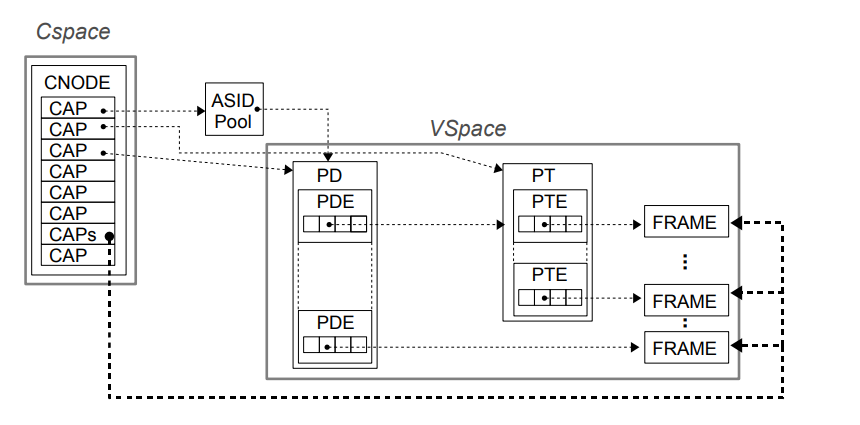
\includegraphics[width=0.7\textwidth]{./Pictures/applicationIntern.png}
	\caption[Internal repersentation of application]{Internal representation of an application in seL4 \cite{sel4}}
	\label{fig:intapp}
	\end{figure}
	
	\item \textbf{Virtual Memory}\\
	A \textit{virtual address space} (VSpace) contains objects for managing virtual memory which largely directly correspond to those of the hardware: \\
	Page Directory, Page Table, Page, ASID Control, ASID Pool
	\item \textbf{Interrupt Objects} \\
	For device driver applications to be able to receive and acknowledge interrupts from hardware devices.
	\item \textbf{Untyped Memory} \\
	Untyped memory objects can be devieded into a group of smaller untyped memory objects. \texttt{Retype()} ist the only method untyped memory capabilities have. It creates a number of new kernel objects and returns capabilities to the new objects if it succeeds. 
	\end{itemize}

	\subsubsection{Memory Allocation Model}
	Important for the seL4 is that all kernel objects must be fully contributed for by capabilities. \\
	At boot time the kernel pre-allocates all the memory required for the kernel to run. This includes the space for kernel code, data and kernel stack. The ressource manager has full authority over the untyped memory (UM) objects, generated by deviding the remain memory into these objects. \\
	A capability to untyped memory can be refined into child capabilities, smaller sized untyped memory blocks or other kernel objects with the retype operation on UM objects. \\
	The creator of an kernel object has full authority over the object. This "full authority" depends on the the object type. \\
	Figure \ref{fig:systarch} shows a sample system architecture in wich a resource manager running at user-level  has the authority to the remaining untyped memory after boot strapping. 
	
	\begin{figure}[ht]
	\centering
		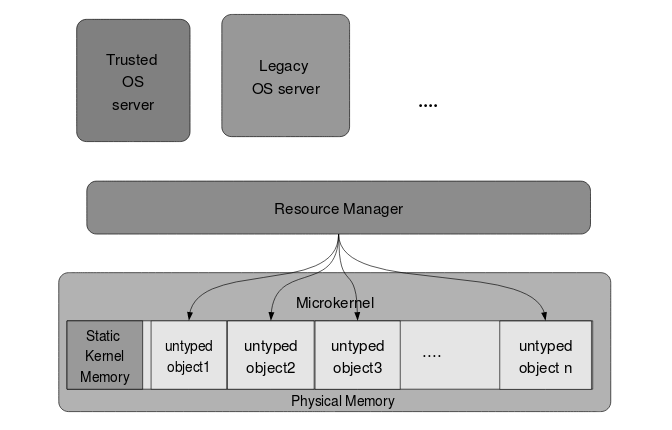
\includegraphics[width=0.7\textwidth]{./Pictures/MemoryAllocation.png}
	\caption[Sample system architecture]{Sample System Configuration \cite{TakeG}}
	\label{fig:systarch}
	\end{figure}	
	
	\newpage
	\subsection{The Take-Grant Model}	
	Protection or Acces control models specify, analyse and implemente secureity policies. 
	The classical Take-Grant Model primary brought in by Lipton and Snyder, 1977 in  \href{https://www.cs.nmt.edu/~doshin/t/s06/cs589/pub/2.JLS-TG.pdf}{%
		"A Linear Time Algorithm for Deciding Subject Security"}.
	\subsubsection{The classical Model}
	The Take-Grant Model \cite{TakeG} represents the system as a directed graph where nodes represent subjects or objects in the system and arcs represent authority. \\ 
	There are graph mutation rlues that represent the system operations that modify the autority distribution.
	The most common rules in the classical model are \textit{take, grant, create} and \textit{remove}. 
	
	\begin{itemize}
	\item \textbf{take rule}: Let S,X,Y be three distinct vertices in the protection graph with an arc, labelled with $\alpha$, from X to Y and one labelled with $\gamma$ from S to X, such that t $\in \gamma.$  
	\begin{figure}[ht]
	\centering
		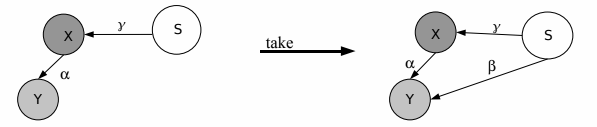
\includegraphics[width=0.7\textwidth]{./Pictures/takeRule.png}
	\caption[take rule]{\textit{Take} adds an edge from S to Y with the label $\beta \subseteq \alpha$. \cite{TakeG}}
	\label{fig:cltake}
	\end{figure}		
	
	\item \textbf{grant rule}:	Let S,X,Y agein be three distinct vertices in the graph with an arc, labelled with  $\alpha$, from S to Y and one labelled with $\gamma$ from S to X, such that g $\in \gamma$. 
	\begin{figure}[ht]
	\centering
		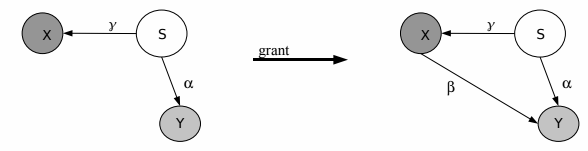
\includegraphics[width=0.7\textwidth]{./Pictures/grantRule.png}
	\caption[grant rule]{\textit{Grant} adds an edge from X to Y with the label $\beta \subseteq \alpha$.  \cite{TakeG}}
	\label{fig:clgrant}
	\end{figure}		
	
	\item \textbf{create rule}: Let S be a vertex in the graph. 
	\begin{figure}[H]
	\centering
		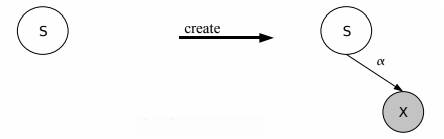
\includegraphics[width=0.5\textwidth]{./Pictures/createRule.png}
	\caption[create rule]{\textit{Create} adds a new node X and an arc from S to X, labelled with $\alpha$. \cite{TakeG}}
	\label{fig:clcreate}
	\end{figure}	
	
	
	\item \textbf{remove rule}: Let S, X be vertices in the graph with an arc from S to X, labelled with $\alpha$. 
	\begin{figure}[ht]
	\centering
		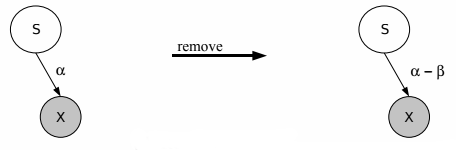
\includegraphics[width=0.5\textwidth]{./Pictures/removeRule.png}
	\caption[remove rule]{\textit{Remove} deletes $\beta$ labels from $\alpha$ or the arc itself if $\alpha - \beta = \lbrace\rbrace$. \cite{TakeG}}
	\label{fig:clremove}
	\end{figure}		
	
	\end{itemize}
	
	
	\subsubsection{Take-Grant specified for the seL4}
	The Take-Grant Model specified in the paper "Noninterference for Operating System Kernels" \cite{TakeG} is a variant of the classical Take-Grant model. \\
	The modification of the \textit{create rule} is the most important one. In the kernel untyped capabilities transfer the authority that has to bei allocated and by the modification adding a new node to the protection graph corresponds to allocation a new object in the concrete kernel. So the only way to apply the create rule is if there is an outgoing arc with \textit{create} authority. The \textit{create} authority is represented by the label \textit{c}. \\
	Also the \textit{remove rule} was modified. It doesn't remove parts of labels. Insted it removes the whole capability, which is the complete arc.\\
	To diminish authority a capability has to be removed and newly created with diminished authority. \\
	The kernel offers an operation called \textit{revoke} wich removes a set of capabilities by mulitple applications of remove. \\
	The goal of the paper "Noninterference for Operating System Kernels" was to show that it is accomblishable to implement isolated subsystems using the mechanisms of the seL4 kernel. \cite{TakeG} \\
	An isolated sybsystem is an collection of connected \textit{entities} enclosed in such a way that authority can neither get in nor out. \\
	The exact specificaton of subsystems and entities follows in Chapter \ref{sec:Formalisation}.
	
	\subsection{Noninterference}
	Noninterference is an enhancement of the information flow model, first published by Goguen and Meseguer in 1982 and updated in 1984. It ensures that objects and subject from different security levels don't interfere with those at other levels.
	The used noninterference formultaion for OS kernels \cite{NonOp} expands von Oheimb's notion of \textit{noninfluence} \cite{Noninf}. \\
	The system is devided in different \textit{domains}. An information flow \textit{policy} $\leadsto$ specifies the allowed information flows between the domains: $u \leadsto v$ if information is allowed to flow from domain u to domain v. \\
	For OS kernels we need an intransitive variant of noninterference, for wich $\leadsto$ can be intransitive. \\
	The traditional Noninterference formulation was enhanced in in two ways: 
	\begin{enumerate}
	\item Traditional formulations presume a static mapping \textbf{\texttt{dom}} from actions to domains. In an OS Kernel the mapping does not only depend on the actions but also on the current system state. So in the used formulation of Noninterference \cite{NonOp} \textbf{\texttt{dom}} also deppendes on the present state \textit{s}. \\
	\texttt{\textbf{dom}\textit{ a s}} equates the domain associated with some action \textit{\texttt{a}} that occurs from state \texttt{\textit{s}}.
	\item Due to the fact that the noninterference formulation in "Noninterference for Operating System Kernels" \cite{NonOp} was preserved by refinement, it is necessary to avert all \textit{domain-visible} nondeterminisms. \\
	Domain-visible nondeterminism is nondeterminism that can be observed by any domain. \\
	From every confidential source of information which is present in the refinement, such nondeterminisms can be abstracted. From this would result the existence of insecure refinements. \\
	\textbf{Lemma 2} \cite{NonOp} determine the restriction of no domain-visible nondeterminisms formally and will be clarified later. 
	\end{enumerate}
	
	\section{Formalisation of the Take-Grant Model}\label{sec:Formalisation}
	\subsection{Capabilities}
	In the Take-Grant model for seL4 \cite{TakeG} the authors waived the usual differentation betwenn subjects and objects and called all kernel objects \textit{entities}. \\ \\
	The entities memory address identifies them and is modeled as a natural number. \\ \\
	{\relsize{-1}
	\textbf{type$\_$synonym} \texttt{ entity$\_$id = nat}} \\ \\
	With each capability a set of rights is associated. There ar four access rights in the system model:	\\ \\
	{\relsize{-1}
	\textbf{datatype} \texttt{ rights = Read | Write | Grant | Create}} \\ 
	\begin{itemize}	
	\item \textit{Read} authorises the reading of information from another entity. 
	\item \textit{Write} authorises the writing of information to another entity. 
	\item \textit{Grant} authorises the passing of a capability to another entity. 
	\item \textit{Create} authorises the creation of new entities, which models the behavior of untyped memory objects. 
	\end{itemize} 
	\vspace{\baselineskip}
	A capability has two fields:
	\begin{enumerate}
	\item An identifier which names an target-entity
	\item A set of rights which defines which system-operations the source-entity is authorisied to perform on the target-entity. 
	\end{enumerate} 
	\vspace{\baselineskip}
	{\relsize{-1}
	\textbf{record} 
	\texttt{	
	\begin{tabular}[t]{ll}
	cap = & entity :: entity$\_$id \\
	      & rights :: rights set
	\end{tabular}} }
	\\ \\ \\
	An entity has a set of capabilities: \\ \\
	{\relsize{-1}
	\textbf{record } \texttt{ 						
	entity = caps :: cap set}} \\ \\
	The systems state includes two flields: 
	\begin{enumerate}
	\item The \texttt{heap}, which stores the entities of the system like an arry form address \texttt{0} up to and excluding \texttt{next$\_$id}.
	\item \texttt{next$\_$id} contains slot for next entity without overlapping with an existing one. 
	\end{enumerate}
	\vspace{\baselineskip}
	{\relsize{-1}	
	\textbf{record}
	\texttt{
	\begin{tabular}[t]{ll}
	state =	& heap :: entity$\_$id $\Rightarrow$ entity \\
			& next$\_$id :: entity$\_$id
	\end{tabular}} }
	\newpage
	\subsection{System Operations}
	The system operations of the seL4 are determined in the data type \texttt{sysOps}. \\ \\
	{\relsize{-1}	
	\textbf{datatype}
	\texttt{
	\begin{tabular}[t]{lll}
	sysOps	&	=	&	SysNoOp entity$\_$id \\
			&	|	&	SysRead	entity$\_$id cap \\
			&	|	&	SysWrite entity$\_$id cap \\
			&	|	&	SysCreate entity$\_$id cap cap \\
			&	|	&	SysGrant entity$\_$id cap cap rights set \\
			&	|	&	SysRemove	entity$\_$id cap cap \\
			&	|	&	SysRevoke entity$\_$id cap
	\end{tabular}}} \\ \\
	The entity$\_$id in each operation is the entity initiating the operation. The first named capability is the one that is being invoked. The second capability for \texttt{SysCreate} points to the target entity for the new capability. For \texttt{SysGrant} it's the passed capability and for \texttt{SysRemove} it's the one that has to be removed. The rights set in \texttt{SysGrant} necessary for the initiating entity to have the option only to transport a subset of the authority it offers to the receiver. 	\\
	The \texttt{diminish} function applies this mask on the given acces rights: \\ \\
	{\relsize{-1}	
	\texttt{
	diminish :: "cap $\Rightarrow$ rights set $\Rightarrow$ cap" \textbf{where} \\
	diminish c R $\equiv$ c$\llparenthesis$rights := rights c $\cap$ \textit{R}$\rrparenthesis$}} \\ \\ \\
	\texttt{legal} defines on what terms any system operation is allowed. \\ \\
	{\relsize{-1}
	\texttt{legal :: "sysOPs $\Rightarrow$ state $\Rightarrow$ bool" \texttt{where}}\\ \\
	\texttt{
	\begin{tabular}{lllll}
	  	&	"legal	&	(SysNoOp e) s	&	=	&	isEntityOf s e" \\
	|	& 	"legal	&	(SysCreate e c$_1$ c$_2$) s	&  =	& (isEntityOf s e $\wedge$ {c$_1$, c$_2$} $\subseteq$ caps$\_$of s e $\wedge$ \\ & & & & Grant $\in$ rights c$_2$ $\wedge$ Create $\in$ rights c$_2$)" \\
	| 	& "legal 	& 	(SysRead e c) s	&	=	&	(isEntityOf s e $\wedge$ c $\in$ caps$\_$of s e $\wedge$ Read \\ & & & & $\in$ rights c)" \\
	|	&	"legal 	&	(SysWrite e c) s&	= 	&	(isEntityOf s e $\wedge$ c $\in$ caps$\_$of s e $\wedge$ Write \\ & & & & $\in$ rights c)" \\
	| 	&	"legal 	&	(SysGrant e c$_1$ c$_2$ r) s & = & (isEntityOf s e $\wedge$  isEntityOf s (entity c$_1$) \\ & & & & $\wedge$ {c$_1$,c$_2$} $\subseteq$ caps$\_$of s e $\wedge$ Grant $\in$ rights c$_1$)" \\
	| 	&	"legal 	&	(SysRemove e c$_1$ c$_2$) s	&  =	& (isEntityOf s e $\wedge$ c$_1$ $\in$ caps$\_$of s e)" \\
	|	&	"legal	&	(SysRevoke e c) s	&	=	&	isEntityOf s e $\wedge$ c $\in$ caps$\_$of s e"
	\end{tabular}}} \\ \\ \\
	\texttt{isEntityOf} tests the existence of an \texttt{entity$\_$id}, \texttt{caps$\_$of} issues the set of all capabilities  contained in the entity with the address \texttt{r} in state \texttt{s}. \\ \\
	The original executions of \texttt{SysRead} and \texttt{SysWrite} don't have an underlying function. For implying the noninterference property I have to include what happens if an entity reads or writes a value from another entity. For this purpose I defined a \texttt{readOperation} and a \texttt{writeOperation}. \\
	The \texttt{step'} and \texttt{step} functions define the execution of a single system operation: \\ \\
	{\relsize{-1}	
	\texttt{step' :: "sysOPs $\Rightarrow$ state $\Rightarrow$ state" \textbf{where}} \\
	\texttt{
	\begin{tabular}{lllll}
		&	"step'	&	(SysNoOp e) s	&	=	&	s" \\
	|	&	"step'	&	(SysRead e c) s	&	=	&	readOperation e c s" \\
	|	&	"step'	&	(SysWrite e c) s &	=	&	writeOperation e c s" \\
	|	&	"step'	&	(SysCreat e c$_1$ c$_2$) s & = & createOperation e c$_1$ c$_2$ s" \\
	|	&	"step'	&	(SysGrant e c$_1$ c$_2$ \textit{R}) s & = & grantOperation e c$_1$ c$_2$ \textit{R} s" \\
	|	&	"step'	&	(SysRemove e c$_1$ c$_2$) s & = & removeOperation e c$_1$ c$_2$ s" \\
	|	&	"step'	&	(SysRevoke	e c) s & =	&	revokeOperation e c s" 
	\end{tabular}} \\ \\
	\texttt{step :: "sysOps $\Rightarrow$ state $\Rightarrow$ state" \textbf{where} \\
	step cmd s $\equiv$ if legal cmd s then step' cmd s else s}} \\ \\
	The new defined functions \texttt{readOperation} and \texttt{writeOperation}: \\ \\
	{\relsize{-1}	
	\texttt{readOperation :: "entity$\_$id $\Rightarrow$ cap $\Rightarrow$ modify$\_$state" \textbf{where}} \\
	\texttt{"readOperation e c s $\equiv$ s$\llparenthesis$ heap := (heap s)(e := $\llparenthesis$caps = caps$\_$of s e, eValue = value$\_$of s (entity c)$\rrparenthesis$)$\rrparenthesis$"}}\\ \\
	{\relsize{-1}	
	\texttt{writeOperation :: "entity$\_$id $\Rightarrow$ cap $\Rightarrow$ modify$\_$state" \textbf{where}} \\
	\texttt{"writeOperation e c s $\equiv$ s$\llparenthesis$ heap := (heap s)(entity c := $\llparenthesis$caps = caps$\_$of s (entity c), eValue = value$\_$of s e|))|)"}}\\ \\
	The rest of the system operation stay as they are: \\ \\
	{\relsize{-1}
	\texttt{createOperation :: "entity$\_$id $\Rightarrow$ cap $\Rightarrow$ cap $\Rightarrow$ modify$\_$state" \textbf{where}} \\
  \texttt{createOperation e c$_1$ c$_2$ s $\equiv$ \\
  \begin{tabular}{ll}
            let & nullEntity = $\llparenthesis$cap = {}, eValue = NULL$\rrparenthesis$ ; \\
                & newCap = $\llparenthesis$entity = next$\_$id s, rights = all$\_$rights$\rrparenthesis$; \\
                & newTarget = $\llparenthesis$caps = {newCap} ∪ caps$\_$of s (entity c$_2$), eValue = NULL$\rrparenthesis$ \\
             in & s$\llparenthesis$heap := (heap s)(entity c$_2$ := newTarget, next$\_$id s := nullEntity), next$\_$id := next$\_$id s+1$\rrparenthesis$"
   \end{tabular} \\ \\ \\
    grantOperation :: "entity$\_$id $\Rightarrow$ cap $\Rightarrow$ cap $\Rightarrow$ rights set $\Rightarrow$ modify$\_$state" \textbf{where} \\
  "grantOperation e c$_1$ c$_2$ \textit{R} s $\equiv$ \\
  s$\llparenthesis$heap := (heap s)(entity c$_1$ := $\llparenthesis$caps = {diminish c$_2$ \textit{R}} $\cup$ caps$\_$of s (entity c$_1$), eValue = value$\_$of s (entity c$_1$)$\rrparenthesis$)$\rrparenthesis$"\\ \\ \\
   removeOperation :: "entity$\_$id $\Rightarrow$ cap $\Rightarrow$ cap $\Rightarrow$ modify$\_$state" \textbf{where} \\
  "removeOperation c$_1$ c$_2$ s $\equiv$ s$\llparenthesis$heap := (heap s)(entity c$_1$ := $\llparenthesis$caps = caps$\_$of s (entity c$_1$) - {c$_2$}, eValue = value$\_$of s (entity c$_1$)$\rrparenthesis$)$\rrparenthesis$"}} \\ \\ \\ 
\newpage
\section{Validation of Confidentiality}
First I tried to validate confidentiality for the different system operations as they are defined in the take-grant-model. With this model it's impossible to decide whether a change of value has been recognized by another domain. \\
In the paper an entity only include a set of capabilites. For my purpose I need the option to access the content of the entities. This ist because the rules for noninterference state that no information is allowed to flow from one domain to another. This includes the information stored in the kernel objects. 
Therefore I extendet the original record \texttt{entity} by adding a \textit{value} modelled by a natural number. \\ \\
My entity type: \\ \\
	{\relsize{-1}
	\textbf{record} 
	\texttt{
	\begin{tabular}[t]{ll}
	entity = & caps :: cap set \\
			 & eValue :: nat 														
	\end{tabular}}} \\ \\ \\
After this change it was feasible to deside confidentiality for this model in the following way.\\ \\
I took one Low-level-Subsystem and one High-level-Subsystem with entities in them and tested for different right-sets and different operations if the confidentiality-property holds. The following shows an example of this approach: \\ 
\begin{itemize}
\item e$\_1 \in$ H, e$_2 \in$ L, c$_1$ $\in$ s,  c$_2$ $\in$ t
\item H equates a High level domain that implements the subsystem 'H'
\item L equates a Low level domain that implements the subsystem 'L'
\end{itemize}
\begin{figure}[H]
\pgfuseimage{WriteGraphic1}
\caption{Confidentiality of Write 1}
\end{figure}
* s $\overset{\text{L}}{\sim}$ t $\Rightarrow$ aquiv$\_$nonin s t L	\\ 
** writeOperation e$_2$ c$_2$ t changes e$\_1$ $\in$ H not e $\in$ L \\
*** writeOperation e$_2$ c$_1$ s = s' $\overset{\text{****}}{=}$ s \\
**** legal(SysRead e$_2$ c$_1$) s = false \\ \\ \\ \\
$\forall$ e$\in$L. \\ 
\begin{tabular}{ll}
& value$\_$of s' e $\overset{\text{***}}{=}$ value$\_$of s e $\overset{\text{*}}{=}$ value$\_$of t e $\overset{\text{**}}{=}$ value$\_$of t' e \\
$\wedge$ & caps$\_$of s' e $\overset{\text{***}}{=}$ caps$\_$of s e $\overset{\text{*}}{=}$ caps$\_$of t e $\overset{\text{**}}{=}$ caps$\_$of t' e \\
$\wedge$ & subSys s' e $\overset{\text{***}}{=}$ subSys s e $\overset{\text{*}}{=}$ subSys t e $\overset{\text{**}}{=}$ subSys t' e
\end{tabular} \\
$\Rightarrow$ aquiv$\_$nonin s' t' L $\Rightarrow$ s' $\overset{\text{L}}{\sim}$ t' \\ \\
\begin{figure}[H]
\pgfuseimage{WriteGraphic2}
\caption{Confidentiality of Write 2}
\end{figure}
* s $\overset{\text{L}}{\sim}$ t $\Rightarrow$ aquiv$\_$nonin s t L	\\ 
** writeOperation e$_2$ c$_1$ s changes e$\_1$ $\in$ H no e $\in$ L \\ 
*** writeOperation e$_2$ c$_2$ t changes e$\_1$ $\in$ H no e $\in$ L \\ \\
$\forall$ e$\in$L. \\
\begin{tabular}{ll}
& value$\_$of s' e $\overset{\text{**}}{=}$ value$\_$of s e $\overset{\text{*}}{=}$ value$\_$of t e $\overset{\text{***}}{=}$ value$\_$of t' e \\
$\wedge$ & caps$\_$of s' e $\overset{\text{**}}{=}$ caps$\_$of s e $\overset{\text{*}}{=}$ caps$\_$of t e $\overset{\text{***}}{=}$ caps$\_$of t' e \\
$\wedge$ & subSys s' e $\overset{\text{**}}{=}$ subSys s e $\overset{\text{*}}{=}$ subSys t e $\overset{\text{***}}{=}$ subSys t' e
\end{tabular} \\
$\Rightarrow$ aquiv$\_$nonin s' t' L $\Rightarrow$ s' $\overset{\text{L}}{\sim}$ t'
\subsection{Redesign of the take-grant-model}
This procedure worked until I came to the remove-operation. There I got the problem, that an entity in the given model is allowed to delete a capability and with that also an object in another domain without any restrictions:
\begin{figure}[H]
\pgfuseimage{RemoveGraphic1}
\caption{No confidentiality for Remove}
\end{figure}
To research into this problem I desided to classify the entities by their types,corresponding to the kernel specification \cite{Manual} \\ 
The following table showes the different object types with their different executable operations and the corresponding take-grant system calls. \\ 
\begin{table}[H]
\begin{tabular}[h]{|l|c|c|}
\hline
Capability Type & Concrete Kernel & protection model \\
\hline
\hline
Untyped & Retype & sequence of \textit{SysCreate} \\
& Revoke & \textit{SysRevoke} \\
\hline
TCB & TreadControl & \textit{SysNoOP, SysGrant} \\
& Exchange Registers & \textit{SystWrite} or \textit{SysRead} \\
& Yield & \textit{SysNoOP} \\
\hline
Synchronous IPC & Send IPC & \textit{SysWrite} or \textit{SysNoOP} \\
(Endpoint) & Wait IPC & \textit{SysRead} \\
& Grant IPC & \textit{SysWrite, SysGrant} or \textit{SysNoOP} \\
\hline
Asynchronous IPC & Send Event & \textit{SysWrite} \\
(AsyncEndpoint) & Wait Event & \textit{SysRead} \\
\hline
CNode & imitate & \textit{SysGrant} \\
& mint & \textit{SysGrant} \\
& Remove & \textit{SysRemove} \\
& Revoke & \textit{SysRevoke} \\
& Move & \textit{SysGrant, SysRemove} \\
& Recycle & \textit{SysRevoke}, sequence of \textit{SysRemove} \\
\hline
VSpace & Install Mapping & \textit{SysGrant} \\
& Remove Mapping & \textit{SysRemove} \\
& Remap & \textit{SysRemove, SysGrant} \\
& initialise & \textit{SysNoOP} \\
\hline
Frame & - & - \\
\hline
InterruptController & Register interrupt & \textit{SysGrant} \\
& Unregister interrupt & \textit{SysRemove} \\
\hline
InterruptHandler & Acknowledge intrrupt & \textit{SysWrite} \\
\hline
seL4 ASID Table & Associate VSpace & \textit{SysNoOP} \\
& Disassociate VSpace & \textit{SysNoOP} \\
\hline
\end{tabular}
\caption{Relationship: operation of concrete kernel $\longleftrightarrow$ of protection model \cite{PhDseL4}}
\end{table}
For the validation I took a subsystem (SS1) of one Domain (D1) an another subsystem (SS2) of second Domain (D2). \\
As mentioned in chapter \ref{sec:KernelObjects} (Kernel Objects), the only communication between Domains goes through \textit{Shared Pages} or \textit{Asynchronous Endpoints}. \\
The following picture shows an example of how the objects and methods can be placed in the domains and how the connection to \textit{Shared Pages} and \textit{Asynchronous Endpoints} is implemented if the information is allowed to flow from Domain 1 to Domain 2.
\begin{figure}[H]
\pgfuseimage{OverviewObjects}
\caption{Objects and Methods in the kernel}
\end{figure}
\subsubsection{Create}\label{sec:Create}
Create corresponds to the \textit{Retype} operation on untyped memory. Each Domain has a own and fixed section of memory. So so UMO for \textit{Retype} is located in the same Domain as the implementing entity. Also the created entity is placed in the same Domain as in the CDT it is a child of the UMO.  \\
The following picture shows 
\begin{flushleft}
\begin{figure}[H]
\pgfuseimage{CreateUMO}
\caption{Confidentiality for Create}
\end{figure}
\end{flushleft}
* s $\overset{\text{D1}}{\sim}$ t $\Rightarrow$ aquiv$\_$nonin s t D1	\\ 
** createOperation e$_2$ c$_1$ c$_2$ t creates e$_3$ $\in$ D2 and does not change or create any e $\in$ D1 \\ \\
$\forall$ e $\in$ D1. \\ 
\begin{tabular}{ll}
& value$\_$of s' e $\overset{\text{**}}{=}$ value$\_$of s e $\overset{\text{*}}{=}$ value$\_$of t e $\overset{\text{**}}{=}$ value$\_$of t' e \\
$\wedge$ & caps$\_$of s' e $\overset{\text{**}}{=}$ caps$\_$of s e $\overset{\text{*}}{=}$ caps$\_$of t e $\overset{\text{**}}{=}$ caps$\_$of t' e \\
$\wedge$ & subSys s' e $\overset{\text{**}}{=}$ subSys s e $\overset{\text{*}}{=}$ subSys t e $\overset{\text{**}}{=}$ subSys t' e
\end{tabular} \\
$\Rightarrow$ aquiv$\_$nonin s' t' D1 $\Rightarrow$ s' $\overset{\text{D1}}{\sim}$ t' \\ \\


	\cleardoublepage
	\begin{thebibliography}{99}

	\bibitem{NonOp}
	T.\ Murray, D.\ Matichuk, M.\ Brassil, P.\ Gammie and G.\ Klein:	\\ 
	\href{http://www.ssrg.nicta.com/publications/nicta_full_text/6004.pdf}{%
		Noninterference for Operating System Kernels}. \\
    International Conference on Certified Programs and Proofs, pp. 126–142, Kyoto, Japan, December, 2012

	\bibitem{TakeG}
	D.\ Elkaduwe, G.\ Klein and K.\ Elphinstone:	\\ 
	\href{http://ts.data61.csiro.au/publications/nicta_full_text/1474.pdf}{%
		Verified Protection Model of the seL4 Microkernel}. \\
   	Technical Report NRL-1474, NICTA, October, 2007
   	
   	\bibitem{sel4}
	J.\ Andronick T.\ Bourke P.\ Derrin D.\ Greenaway D.\ Elkaduwe, G.\ Klein and K.\ Elphinstone R.\ Kolanski D.\ Matichuk T.\ Sewell S.\ Winwood:	\\ 
	\href{https://sel4.systems/Info/Docs/seL4-spec.pdf}{%
		Abstract Formal Specification of the seL4/ARMv6 API}. \\
   	Version 1.3
   	
   	\bibitem{Noninf}
	D.\ von Oheimb	\\ 
	\href{https://pdfs.semanticscholar.org/21ea/6c722535ed0a22175187796b43c114e14ee8.pdf}{%
		Information flow control revisited: Noninfluence = Noninterference + Nonleakage}. \\
   	In \textit{9th ESORICS}, volume 3193 of \textit{LNCS}, pages 225-243, 2004.
   	
   	 	\bibitem{PhDseL4}
	D.\ Elkaduwe:	\\ 
	\href{https://ts.data61.csiro.au/publications/papers/Elkaduwe:phd.pdf}{%
		A Principled Approach To Kernel Memory Management}. \\
   	PhD Thesis, UNSW CSE, Sydney, Australia, March, 2010

	\bibitem{Manual}
	M.\ Grosvenor and A.\ Walker:	\\ 
	\href{http://sel4.systems/Info/Docs/seL4-manual-latest.pdf}{%
		seL4 Reference Manual}. \\
   	Version 10.0.0
\end{thebibliography}
	
\end{document}